\documentclass[letterpaper,12pt]{article}
\usepackage[utf8]{inputenc}
\usepackage[T1]{fontenc}
\usepackage{tgtermes} %%%font
\usepackage{geometry}
\usepackage{amsmath}
\usepackage{float}
\usepackage{graphicx}
\usepackage{subcaption}
\usepackage{amssymb}
\usepackage{adjustbox}
\usepackage{wrapfig} %%imagen envuelta por un texto
\usepackage{xcolor}
\usepackage{fancyhdr}

\title {\textbf{Cálculo multivariable}}
\author{Deniso Xocuis}
\date{10 de junio del 2023}
\geometry{top=2cm, bottom=2cm, left=2cm, right= 2cm} %%margen
\graphicspath{{images/}}
\parindent=0pt

\begin{document}
\maketitle
\thispagestyle{empty}
\newpage
\setcounter{page}{1}
\pagestyle{headings}

%%%%%%%%%%%%%%%%%%%%%%%%%%%%%%%%%%%%%%%%%%%%%%%%%%%%%%%%%%%%%%%%%%%%%%%%%%%%
\begin{sloppypar} 
\section{Función de varias variables}

\begin{center}
    \textbf{\textcolor[rgb]{0.3,0.6,0.7}{Función de una variable}} \textit{(1 variable de entrada, 1 de salida)}:
    \vspace{0.3cm}\\
    $f(x) = x^2 + 1$ donde $f : \mathbb{R} \rightarrow \mathbb{R} $
    \vspace{0.3cm}\\
    \textbf{\textcolor[rgb]{0.3,0.6,0.7}{Función de dos variables}} \textit{(2 variables de entrada, 1 de salida)}:
    \vspace{0.3cm}\\
    $f(x,y) = y^2 - x$ donde $f : \mathbb{R}^{2} \rightarrow \mathbb{R} $
\end{center}
\subsection{Definición formal de una función de dos variables}
\textcolor[rgb]{0.3,0.6,0.7}{Definición (en matemática)}
\vspace{0.3cm}\\
\textit{Una función f de dos variables es una regla que le asigna a cada par ordenado de números reales (x,y) un único número real que se denota con f(x,y)}
Aquellas funciones que contienen más de una variable independiente, la mayoría de los modelos matemáticos de sistemas físicos están en función de dos o más variables

\hspace{0.5cm} \textit{Los pares ordenados (x,y) pertenecen al \textbf{dominio} de la función. El conjunto de todos los valores que toma f(x,y) es el \textbf{rango} de la función} %break es salto de página

\begin{center}
    $(x,y) \in \mathbb{R}^2$
    
    $f(x,y) \in \mathbb{R}^2$ 

    \textit{Se acostumbra a indicar a los valores que toma la función con la variable z, es decir, z = }
\end{center}

Ejemplos:
\begin{enumerate}
    \item V(r,h) = $\pi r^2h$
        \vspace{0.3cm}\\
         $\displaystyle \frac{\partial v}{\partial r} , \frac{\partial V}{\partial h}$
    \item W(f,d) = F*d 
        \vspace{0.3cm}\\
        $\displaystyle \frac{\partial W}{\partial F} \longrightarrow\frac{J}{N}; \frac{\partial W}{\partial d} \longrightarrow \frac{J}{m}$
    \item $E_c(m,v) = \displaystyle \frac{1}{2} mv^{2}$
        \vspace{0.3cm}\\
        $\displaystyle \frac{\partial E_c}{\partial m} \longrightarrow \frac{J}{kg}; \frac{\partial E_c}{\partial v} \longrightarrow \frac{J}{\frac{m}{s}} \longrightarrow \frac{J*s}{m}$
    \item W = $x^2 + y^2 + z^2 $
        \vspace{0.3cm}\\ 
        $\displaystyle \frac{\partial w}{ \partial x} = 2x$
        \vspace{0.3cm}\\ 
        $\displaystyle \frac{\partial w}{ \partial y} = 2x$
        \vspace{0.3cm}\\ 
        $\displaystyle \frac{\partial w}{ \partial z} = 2x$
\end{enumerate}

\subsection{Dominio de una función de dos variables}
$$f(x,y) = \frac{1}{x - y}$$
La función no existe si el denominador es cero, la única forma donde esto ocurra es si "x" y "y" son iguales, por lo tanto: 

$$A = \{(x,y)\in \mathbb{R}^{2} \mid x \neq y \} $$

\subsection{Gráfica de una función de dos variables}
$f(x,y) = y^2 - x$
\vspace{0.3cm}\\
$f(2,1) = -1$ donde (2,1,-1) es (x,y,z), esto quiere decir que se gráfica en 3D, también podemos concluir que z = f(x,y)
\vspace{0.3cm}\\
\textcolor[rgb]{0.3,0.6,0.7}{Definición:}
\vspace{0.3cm}\\
\textit{La gráfica de una función de dos variables es el conjunto de puntos (x,y,z) de $\mathbb{R}^3$ tales que, para cada (x,y,z):}

\hspace{0.5cm}\textit{(x,y) pertenece al dominio de la función, z es el valor del \textbf{rango}}

\break \section{Trazas}
Una traza es la curva que aparece tras hacer la intersección entre la superficie que necesitamos averiguar y planos. 

En la siguiente superficie al intersectarla con un plano, aparece una parábola.

\begin{figure}[H]
    \centering
    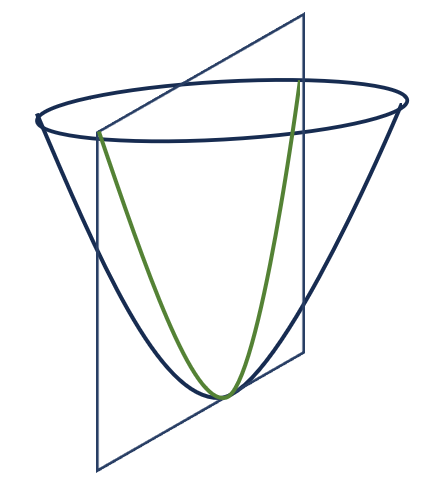
\includegraphics[width=0.4\linewidth]{images/trazas.png}
    \caption{superficie con traza}
\end{figure}

\subsection{\textbf{Ecuación del plano xy}}

z tiene que ser cero, es decir, si tenemos un punto (x,y,z) y le agregamos esa condición, descubrimos la traza xy

\begin{figure}[H]
    \centering
    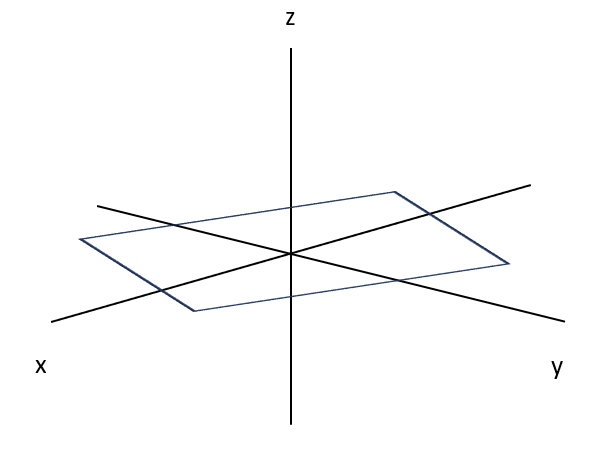
\includegraphics[width=0.4\textwidth]{images/plano xy.png}
    \caption{plano xy}
\end{figure}

\break \subsection{\textbf{Ecuación del plano yz}}
Existe la condición x=0, si por alguna razón este plano está un poco más atrás hasta un punto (-3, por ejemplo) x=-3

\begin{figure}[H]
    \centering
    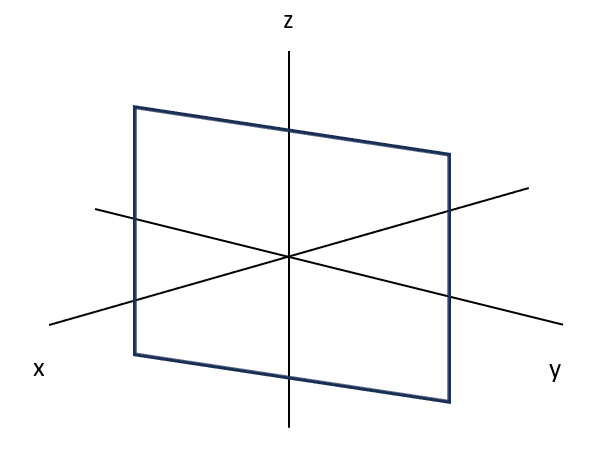
\includegraphics[width=0.4\textwidth]{images/plano yz.png}
    \caption{plano xy}
\end{figure}

\subsection{\textbf{Ecuación del plano xz}}
Tomando la lógica anterior de las otras ecuaciones, concluimos que existe la condición y=0
\begin{figure}[H]
    \centering
    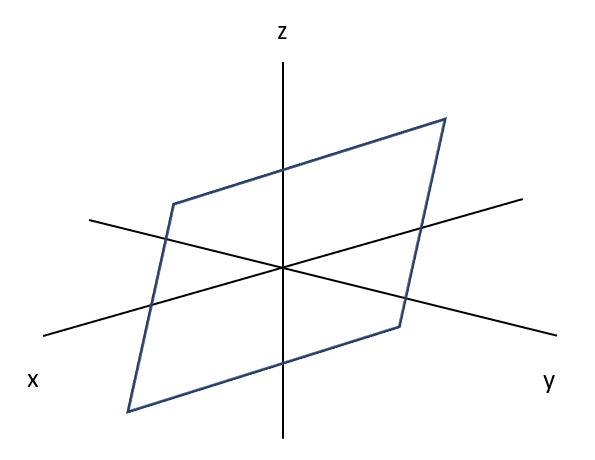
\includegraphics[width=0.4\textwidth]{images/plano xz.png}
    \caption{plano xz}
\end{figure}

\section{Uso de trazas}
\begin{center}
    xz $\longrightarrow$  y=0

    xy $\longrightarrow$ z=0

    yz $\longrightarrow$ x=0
\end{center}

¿Para qué nos sirve entender esto?, si existe una función tal que z = f(x,y) = $x^2 + y^2$ podemos pensar que son dos parábolas pero ¿de qué forma y dirección están posicionadas? las trazas nos dice y nos refleja exactamente la forma de graficar en un plano 3D 

\begin{figure}
    \centering
    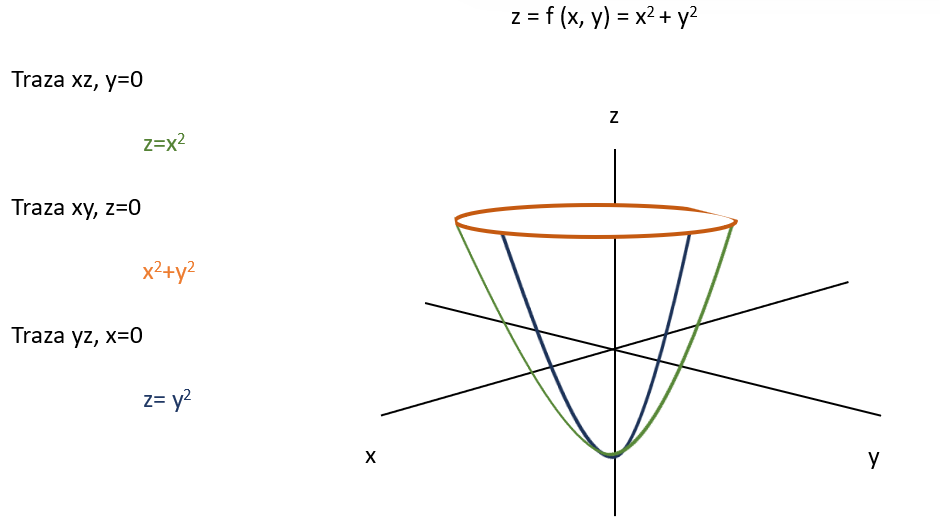
\includegraphics[width=0.8\textwidth]{images/usotraza.png}
\end{figure}

\section{Curvas de nivel}
Intersección entre el plano y la superficie (función), comúnmente se acostumbra a abajarla en el plano xy 

Una curva de nivel es fijar la salida de la función a una constante, el resultado es la intersección con una superficie. Si las curvas están muy pegadas, la superficie crece abruptamente, del lado contrario sucede si las curvas están separadas

\subsection{Función de tres variables}
\begin{center}
    $f(x,y,z) = x^2 - 3y + 2z -1$ donde $f : \mathbb{R}^3 \rightarrow \mathbb{R} $
\end{center}

No se puede graficar una función que sea más de dos variables, se pueden estudiar analíticamente pero no representar en un plano.

\subsection{Función de n-variables}
\begin{center}
    $f(x_1, x_2, ..., x_n)$ donde $f : A \subset \mathbb{R}^{n} \rightarrow \mathbb{R}$
\end{center}

\section{Límites y continuidad de funciones de dos o más variables}
$$\lim_{(x,y) \to (0,0)}  = f(x,y) = L$$

$$f : \mathbb{R}^{n} \rightarrow \mathbb{R}^{n}$$

y = mx

Si las variables de los puntos se acercan a un valor en concreto (dentro de la superficie), el límite existe. Existen infinitas formas de acercarnos a un valor, es decir, no podemos comprobar los infinitos laterales de un punto porque no se puede.

En casos prácticos, no vamos a comprobar la existencia, sino, la noexistencia.



\subsection{Límites laterales}
Hay muchas formas de aproximarse al punto donde (x,y) tiende, este debe ser el mismo para cualquier trayectoria. c: 

\subsection{Cambio de variable}
$$\lim_{(x,y) \to (0,0)}  = \frac{x + y + 1}{x^2 - 4x + y + 7}$$

u = x - 2 $\rightarrow$ u + 2 = x

v = y + 3 $\rightarrow$ v - 3 = y

sustituyendo y simplificando nos queda la expresión: 

$$\lim_{(u,v) \to (0,0)} = \frac{u + v}{u^2 + v}$$

sacando los límites laterales: 

$$ \displaystyle  \lim_{(u) \to (0)} = \frac{u + mu}{u^2 + mu} = \frac{1 + m}{m}$$

Este valor depende de m $\therefore$ el \textit{límite no existe.}

\subsection{Trayectorias que se aproximen al ($x_{0},y_{0}$)}
\begin{figure}
    \centering
    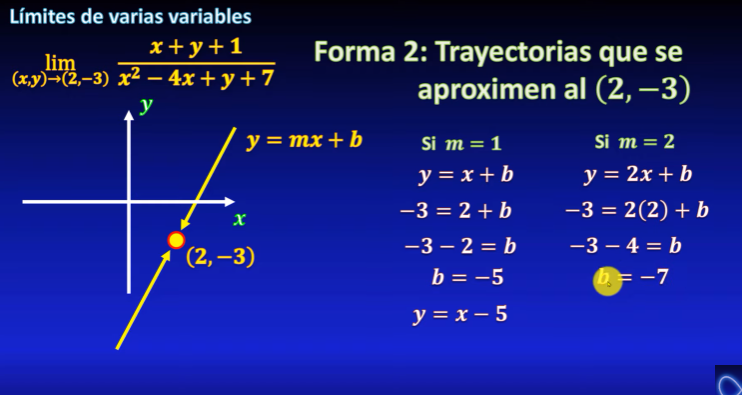
\includegraphics{images/Captura de pantalla 2023-07-06 192610.png}
\end{figure}
\newpage

\section{Derivadas parciales}

$$z = 4x^2y^3 - 3x - 2y + 7$$
\vspace{0.3cm}\\
$\displaystyle \frac{dz}{dx} = f_x \longrightarrow f_x = 8xy^3 - 3$
\vspace{0.3cm}\\ 
$\displaystyle \frac{dz}{dy} = f_y \longrightarrow f_y = 12x^2y^2 - 2 $
\vspace{0.3cm}\\ 
$f_{xx} = 8y^3$
\vspace{0.3cm}\\ 
$f_{yy} = 24x^2y$
\vspace{0.3cm}\\ 
$f_{xy} = 24xy^2 (derivando f_{x})$
\vspace{0.3cm}\\ 
$f_{yx} = 24xy^2$ (tiene que ser igual que $f_{xy}$)

\end{sloppypar}
\end{document}